\chapter{\separake: Sound Source Separation with Echoes}\label{chap:separake}

\marginpar{%
\footnotesize
Source separation, echoes, room geometry, NMF, multi-channel.
}
\newthought{Synopsis} It is commonly believed that multipath hurts various audio processing algorithms.
At odds with this belief, we show that multipath in fact helps sound source separation,
even with very simple propagation models. Unlike most existing methods,
we neither ignore the room impulse responses, nor we attempt to estimate them fully.
We rather assume to know the positions of a few virtual microphones generated by
echoes and we show how this gives us enough spatial diversity to get a performance
boost over the anechoic case. We show improvements for two standard algorithms---one that
uses only magnitudes of the transfer functions, and one that also uses the phases.
Concretely, we show that multi-channel non-negative matrix factorization aided with
a small number of echoes beats the vanilla variant of the same algorithm,
and that with magnitude information only, echoes enable separation where it was previously impossible.
% \section{Introduction}

% \subsection{Literature review: an acoustic perspective}
% Bibliography with respect to sound propagation

% \subsection{Literature review an algorithmic perspective}
% Bibliography with respect to learning and knowledge approaches

% \section{Background in SSS}

% \newthoughtpar{SSS by NMF}

% \newthoughtpar{NMF using Multiplicative-Updates (MU-NMF)}

% \newthoughtpar{NMF using Expectation-Maximization (EM-NMF)}

% \section{\separake: SSS with echoes}

% \section{Experimental evaluation}

% \section{Conclusion}


\section{Introduction}

Source separation algorithms can be grouped according to how they deal with sound propagation:
those that ignore it \cite{le2015deep}, those that assume a single anechoic path \cite{rickard2007duet},
those that model the room transfer functions (TFs) entirely \cite{ozerov2010multichannel,nugraha2016multichannel},
and those that attempt to separately estimate the contribution of the early echoes and the contribution of the late tail \cite{leglaive2015multichannel}.
In this paper we propose yet another route: we assume knowing the locations of a few walls relative to the microphone array,
which enables us to exploit the associated \textit{virtual microphones}.
This assumption is easy to satisfy in living rooms and conference rooms, but the corresponding model incurs a significant mismatch with respect to the complete reverberation.
We show that it nonetheless gives sizable performance boosts while being simple to estimate.
The approach we propose is reminiscent of acoustic rake receivers \cite{Dokmanic:2015dr};
we thus call it \separake.

A typical setup is illustrated in Figure \ref{fig:separake:setup}.
We consider $J$ sources emitting from $J$ distinct directions of arrival (DOAs) $\set{\theta_j}_{j=1}^J$,
and an array of $M$ microphones.
The array is placed close to a wall or a corner.
There are two reasons why this is useful:
first, it makes echoes from the nearby walls significantly stronger than all other echoes;
second, it ensures that the resulting virtual array (real and virtual microphones) is compact.
The latter justifies the far field assumption which in turn simplifies exposition.

\begin{figure}
    \centering
    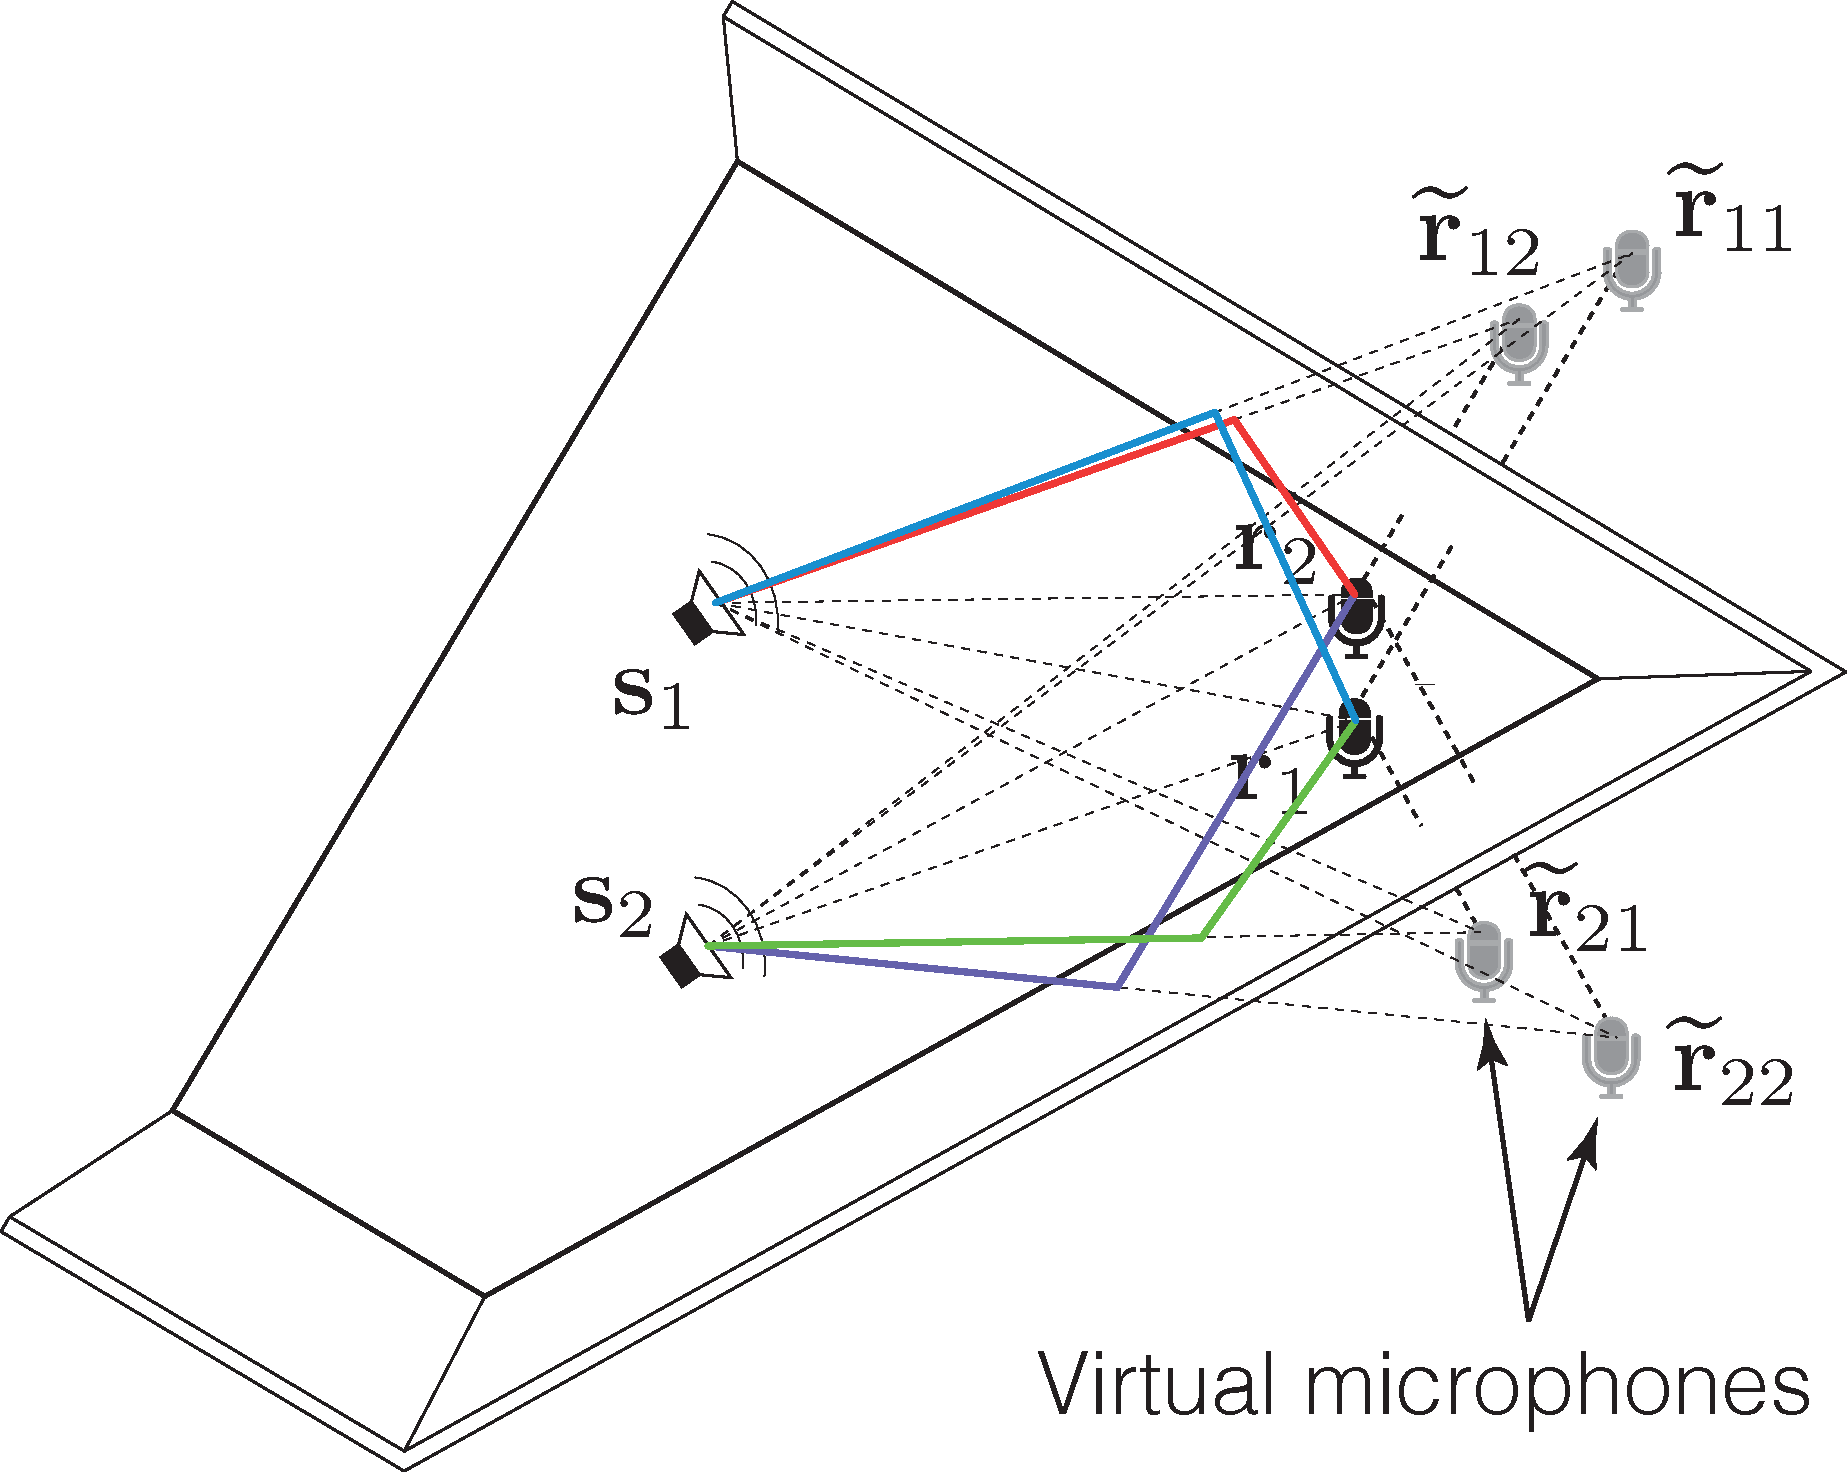
\includegraphics[width=.7\linewidth]{separake/separake.pdf}
    \caption{Typical setup with two speakers recorded by two microphones. The illustration shows the virtual microphone model (grey microphones) with direct sound path (dotted lines) and resulting first-order echoes (colored lines)}
    \label{fig:separake:setup}
    \vspace{-0mm}
\end{figure}

Real and virtual microphones form dipoles with diverse frequency-dependent directivity patterns.
Our goal is to design algorithms which benefit from this known spatial diversity.


Echoes have been used previously to enhance various audio processing tasks.
It was shown that they improve indoor beamforming \cite{Dokmanic:2015dr, Scheibler:2015ii, RobinThesis},
aid in sound source localization \cite{Ribeiro:2010uj},
and enable low-resource microphone array self-localization \cite{Dokmanic:2016gu}.
They have, however, rarely been analyzed in the context of source separation with non-negative source models.

\subsection{Our Goal and Main Findings}

Our emphasis here is different than that in \cite{leglaive2015multichannel}.
Rather than fitting the echo model, we aim to show that separation in the presence of echoes is in fact better than separation without echoes.
We ask the following questions:
\begin{enumerate}
    \item Is speech separation with echoes fundamentally easier than speech separation without echoes?
    Are there specific settings where this is true or false?
    \item Is it necessary to fully model the reverberation or can we get away with a geometric perspective where we know the locations of a few virtual microphones?
\end{enumerate}
To answer these questions we set up several simple experiments.
We take two standard, well-understood multi-channel source separation algorithms which estimate the channel (the TFs),
and instead of updating the channel estimate we simply fix it to the TFs of real and a few virtual microphones.
The first algorithm---non-negative matrix factorization (NMF) via multiplicative updates (MU)---only uses the magnitudes of the transfer functions,
while the second one---expectation maximization (EM)---also uses the phases.
In this initial investigation we look at the (over)determined case ($J \leq M$),
leaving the analysis of the undetermined case to future work. Our findings can be summarized as follows:
\begin{itemize}
    \item (MU) With magnitudes only, multi-channel anechoic separation is hardly any better than single-channel separation:
    as the magnitude of the transfer functions is the same at all microphones, channel modeling offers no diversity.
    The situation is different in rooms where the direction-dependent magnitude of TFs varies significantly from microphone to microphone.
    \textit{We show that replacing the transfer functions with a few echoes (even just one) gives significant performance gains compared to not modeling the TFs at all,
    but also that it does better than learning the TFs through multiplicative updates.}
    \item (EM) With both phases and magnitudes, anechoic separation will be near-perfect since it corresponds to a determined linear system.
    Therefore, any uncertainty from imperfections in channel modeling will make things worse.
    \textit{Surprisingly, approximating the TFs with one echo matches learning them through EM updates and using more outperforms it.}
\end{itemize}
For a sneak peak at the gains, fast forward to Figure \ref{fig:separake:results}.


% \section{Modeling}

% Suppose $J$ sources emit inside the room and we have $M$ microphones.
% Each microphone receives
% \[
%     y_m(t) = \sum_{j = 1}^J c_{jm}(t),
% \]
% with $c_{jm}$ being the spatial image of the $j$th source at the $m$th microphone.
% Spatial images are given as
% \[
%     c_{mj}(t) = (x_j \conv h_{jm})(t),
% \]
% where $h_{jm}$ is the room impulse response between the source $j$ and microphone $m$.
% The room impulse response is a central object in this paper. We model it as
% \[
%     h_{jm}(t) = \sum_{k = 0}^K \alpha_{jm}^k \delta(t - t_{jm}^k) + \epsilon_{jm}(t),
% \]
% where the sum comprises the line-of-sight propagation and the earliest $K$
% echoes we want to account for (at most 6 in this paper),
% while the error term $\epsilon_{jm}(t)$ collects later echoes and the tail of the reverberation.
% We do not assume $e_{jm}(t)$ to be known.
% We assume that the sources are in the far field of real and virtual microphones so the
% times $t_{jm}^k$ depend only on the source DOAs which we assume are known.
% Assuming $K$ echoes per source are known, we can form an approximate TF from source $j$ to microphone $m$,
% \begin{equation}
%     \label{eq:separake:approx_tf}
%     \wh{H}_{j,m}(e^{j\omega}) = \sum_{k=0}^K \wh{\alpha}_{jm}^k e^{-i \omega \hat{t}_{jm}^k}.
% \end{equation}
% %The far field assumption implies that only the relative arrival times are known so we can arbitrarily fix the delay of the direct path to zero. In addition, we assume all walls to be spectrally flat and that $\alpha_{jm}^k$ are known up to a scaling (i.e. $a_{jm}^0 = 1$).
% We only assume relative arrival times and amplitudes to be known,
% that is $\hat{t}_{jm} = t_{jm}^k - t_{jm}^0$ and $\wh{\alpha}_{jm}^k = \alpha_{jm}^k / \alpha_{jm}^0$, respectively.
% In practice, these parameters can be estimated \cite{RemaggiThesis}.
% In addition, we assume all walls to be spectrally flat in the frequency range of interest.

% As usual, we process by frames. In the short-time Fourier transform (STFT) domain the $m$th microphone signal reads
% \begin{equation}
%     \label{eq:separake:stft_mixing}
%     Y_m[f,n] = \sum_{j = 1}^J \wh{H}_{jm}[f] X_{j}[f,n] + B_m[f,n]
% \end{equation}
% %
% with $f$ and $n$ being the frequency and frame index, $X_{j}[f,n]$ the STFT of the $j$th source signal, and $B_m[f,n]$ a term including noise and model mismatch. It is convenient to group the microphone observations in vector form,
% % Equation \eqref{eq:stft_mixing} can be written in matrix--vector form as
% \begin{equation}
%     \vY[f,n] = \wh{\mH}[f] \, \vX[f,n] + \vB[f,n].
% \end{equation}
% where $\vY[f, n] = \big[ \, Y_m[f, n] \, \big]_m$, $\wh{\mH}[f] = \big[ \, \wh{H}_{jm}[f, n] \, \big]_{m,j}$, $\vX[f, n] = \big[ \, X_j[f, n] \, \big]_j$, and $\vB[f, n] = \big[ \, B_m[f, n] \, \big]_m$.
% Let the squared magnitude of the spectrogram of the $j$th source be $\mP_j = \big[ \abs{X_{j}[f, n]}^2 \big]_{fn}$. We postulate a non-negative factor model for $\mP_j$:
% %
% \begin{equation}
%     \label{eq:nmf_model}
%     \mP_j =  \mD_j \mZ_j,
% \end{equation}
% where $\mD_j$ is the non-negative \textit{dictionary}, and the latent variables $\mZ_j$ are called \textit{activations}.
% Source separation can then be cast as an inference problem in which we maximize the likelihood of the observed $\vY$ over all possible non-negative factorizations \eqref{eq:nmf_model}. This normally involves learning the channel (frequency-domain mixing matrices). Instead of learning, we fix the channel to the earliest few echoes.

% \section{Source Separation by NMF}

% To evaluate the usefulness of echoes in source separation, we modify the
% multi-channel NMF framework of Ozerov and F\'{e}votte \cite{ozerov2010multichannel} as follows.
% First, we introduce a dictionary learned from available training data.
% We explore both speaker-specific and universal dictionaries \cite{Sun:2013co}.
% Speaker-specific dictionaries can be beneficial when speakers are known in advance.
% Universal dictionary is more versatile but gives a weaker regularization prior.
% Second, rather than learning the TF from the data, we use the approximate model of \eqref{eq:approx_tf}.
% In the following we briefly describe the two algorithms used.

% \subsection{NMF using Multiplicative Updates (MU-NMF)}\label{sec:mu}

% Multiplicative updates for NMF only involve the magnitudes and are simpler than the EM updates.
% The updates are guaranteed non-negative as long as the intitialization is.
% They have been originally proposed by Lee and Seung \cite{Lee:2001ti}.
% We use the Itakura-Saito divergence \cite{Fevotte:2011af} between the observed multi-channel squared magnitude spectra $\mV_m = [|Y_m[f,n]|^2]_{fn}$ and their non-negative factorizations,
% \begin{equation}
%     \label{eq:mu_nmf_model}
%     \wh{\mV}_m = \sum_{j=1}^{J} \diag(\vQ_{jm}) \mD_j \mZ_j, \quad m=1,\ldots,M
% \end{equation}
% where $\vQ_{jm} = \big[ \, |\wh{H}_{jm}[f]|^2 \,\big]_f$ is the vector of squared magnitudes of the approximate TF between microphone $m$ and source $j$.
% We add an $\ell_1$-penalty term to promote sparsity in the activations due to the potentially large size of the universal dictionary~\cite{Sun:2013co}.
% The cost function is thus
% \begin{equation}
%     C_{\mathsf{MU}}(\mZ_j) = \sum_{mfn} d_{\mathsf{IS}}(V_{m}[f,n] | \wh{V}_{m}[f,n])
%     + \gamma \sum_j \| \mZ_j \|_1,
% \end{equation}
% where $d_{\mathsf{IS}}(v | \hat{v}) = \frac{v}{\hat{v}} - \log \frac{v}{\hat{v}} - 1$.
% By adapting the original MU rule derivations from Ozerov and F\'{e}votte, we obtain the following regularized MU update rule:
% \begin{align}
%     \mZ_j \gets \mZ_j \odot \frac{\sum_m (\diag(\vQ_{ij}) \mD_j)^\top \left(\mV_j \odot \wh{\mV}_j^{-2}\right)}{\sum_m(\diag(\vQ_{ij}) \mD_j)^\top \wh{\mV}_j^{-1} + \gamma},
% \end{align}
% where multiplication $\odot$, power, and division are element-wise.

% Importantly, neglecting the reverberation (or working in the anechoic regime) leads to a constant $\vQ_{jm}$ for all $j$ and $m$. A consequence is that the MU-NMF framework breaks down with a universal dictionary. Indeed, \eqref{eq:mu_nmf_model} becomes the same for all $m$,
% $
%     \wh{\mV}_m = \sum_{j} \mD \mZ_j = \mD \sum_j \mZ_j,
% $
% so even with the correct atoms identified, we can assign them to any source without changing
% the value of the cost function. Therefore, anechoic multi-channel separation with a universal dictionary cannot work well. This intuitive reasoning is corroborated by numerical experiments in Section \ref{sec:results}.
% %The problem is overcome by the EM-NMF algorithm which keeps the channel phase and is thus able to exploit the phase diversity across the array. Of course, in line with the message of this paper, it is also overcome by using echoes.
% Of course, in line with the message of this paper, this problem is overcome by using echoes.

% \subsection{NMF using Expectation Maximization (EM-NMF)}

% Unlike the MU algorithm that independently maximizes the log-likelihood of TF magnitudes, EM-NMF maximizes the joint log-likelihood over all complex-valued channels~\cite{ozerov2010multichannel}. Hence, it takes into account observed phases.
% Each source $j$ is modeled as the sum of components with complex Gaussian priors of the form $c_{k}[f,n]\sim \mathcal{C}\mathcal{N}\Big(0, d_{fk}z_{kn}\Big)$ such that
% \begin{equation}
%     X_j[f,n] \sim \mathcal{C}\mathcal{N}\left(0, (\mD_j\mZ_j)_{fn}\right),
% \end{equation}
% and the magnitude spectrum $\mP_j$ of \eqref{eq:nmf_model} can be understood as the variance of source $j$.
% Under this model, and assuming uncorrelated noise, the microphone signals also
% follow a complex Gaussian distribution with covariance matrix
% \begin{equation}
%     \mSigma_{\vY}[f,n] = \wh{\mH}[f] \, \mSigma_\vX[f,n] \, \wh{\mH}^H[f] + \mSigma_\vB[f,n],
% \end{equation}
% and the negative log-likelihood of the observed signal is
% \begin{equation}\nonumber %label{eq:EMcriterion}
% \resizebox{\linewidth}{!}{
%     $C_{\mathsf{EM}}(\mZ_j) = \sum\limits_{fn} \trace\left(\vY[f,n]\vY[f,n]^H\mSigma_{\vY}^{-1}[f,n]\right) \\
%     + \log\det\mSigma_{\vY}[f,n].$
%     }
% \end{equation}
% This quantity can be efficiently minimized using the EM algorithm proposed in~\cite{ozerov2010multichannel}. We modify the original algorithm by fixing the source dictionaries $\mD_j$ and the early-echo channel model $\wh{\mH}[f]$ throughout the iterations.
% Since adding sparsity priors is not straightforward in the EM framework, the universal dictionary was left for future work.